\PassOptionsToPackage{hyphens}{url}
\documentclass[aspectratio=169]{beamer}
% \documentclass[aspectratio=169, handout]{beamer}

\usepackage{sty/slides}
\usepackage{sty/sigma/sigma}

\usepackage{sty/math}
\usepackage{sty/stat}
\usepackage{sty/algo}
\usepackage{sty/code}

\usepackage{csquotes}

\newcommand{\knapsacklp}[2]{
    \begin{align*}
        \min \qquad        & #1 \\
        \text{s.t.} \qquad & #2 \\
                           & 0 \le x_i \le 1
    \end{align*}
}

\tikzset{
    invisible/.style={opacity=0},
    visible on/.style={alt={#1{}{invisible}}},
    alt/.code args={<#1>#2#3}{\alt<#1>{\pgfkeysalso{#2}}{\pgfkeysalso{#3}}},
}

\usepackage[style=verbose, backend=biber]{biblatex}
\addbibresource{refs.bib}

\title{Graph Optimization with Mixed Integer Programming}

\author{Ian Chen}
\date{}

% \subtitle{}
% \institute{University of Illinois Urbana-Champaign}

\begin{document}

\begin{frame}
    \titlepage
\end{frame}

\begin{frame}{Optimization problems in the wild}
    \begin{itemize}
        \item Recommendation systems
        \item Resource allocation
        \item Unsupervised learning
        \item \textbf{Traffic engineering (routing)}
        \item \textbf{Traveling salesman}
    \end{itemize}
\end{frame}

\begin{frame}{Outline}
    \tableofcontents
\end{frame}

\section{Traffic engineering}
\frame{\tableofcontents[currentsection]}

\begin{frame}{Traffic engineering}
    \centering
    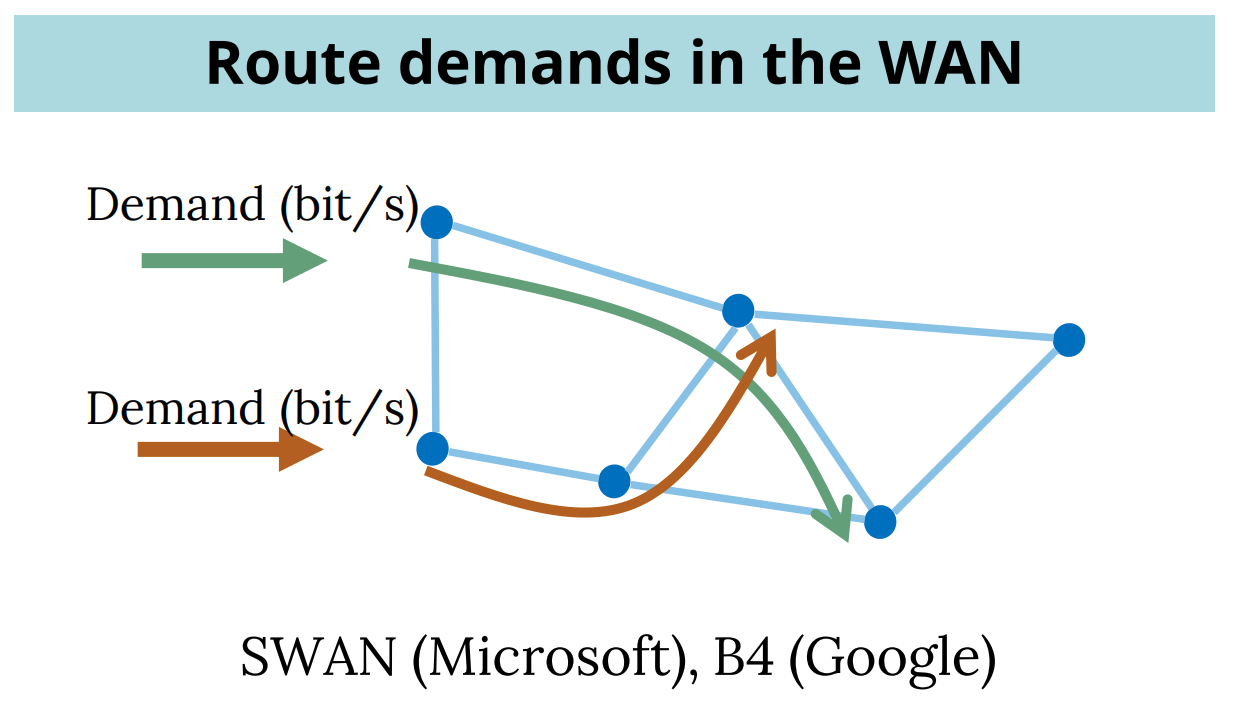
\includegraphics[width=0.9\textwidth]{figs/namyar2024solving-1.png}

    \blfootcite{namyar2024solving}
\end{frame}

\begin{frame}{Traffic engineering (cont.)}
    \begin{itemize}
        \item Servers $\ll$ racks $\ll$ aggregation node $\ll$ $\ldots$
    \end{itemize}

    \centering
    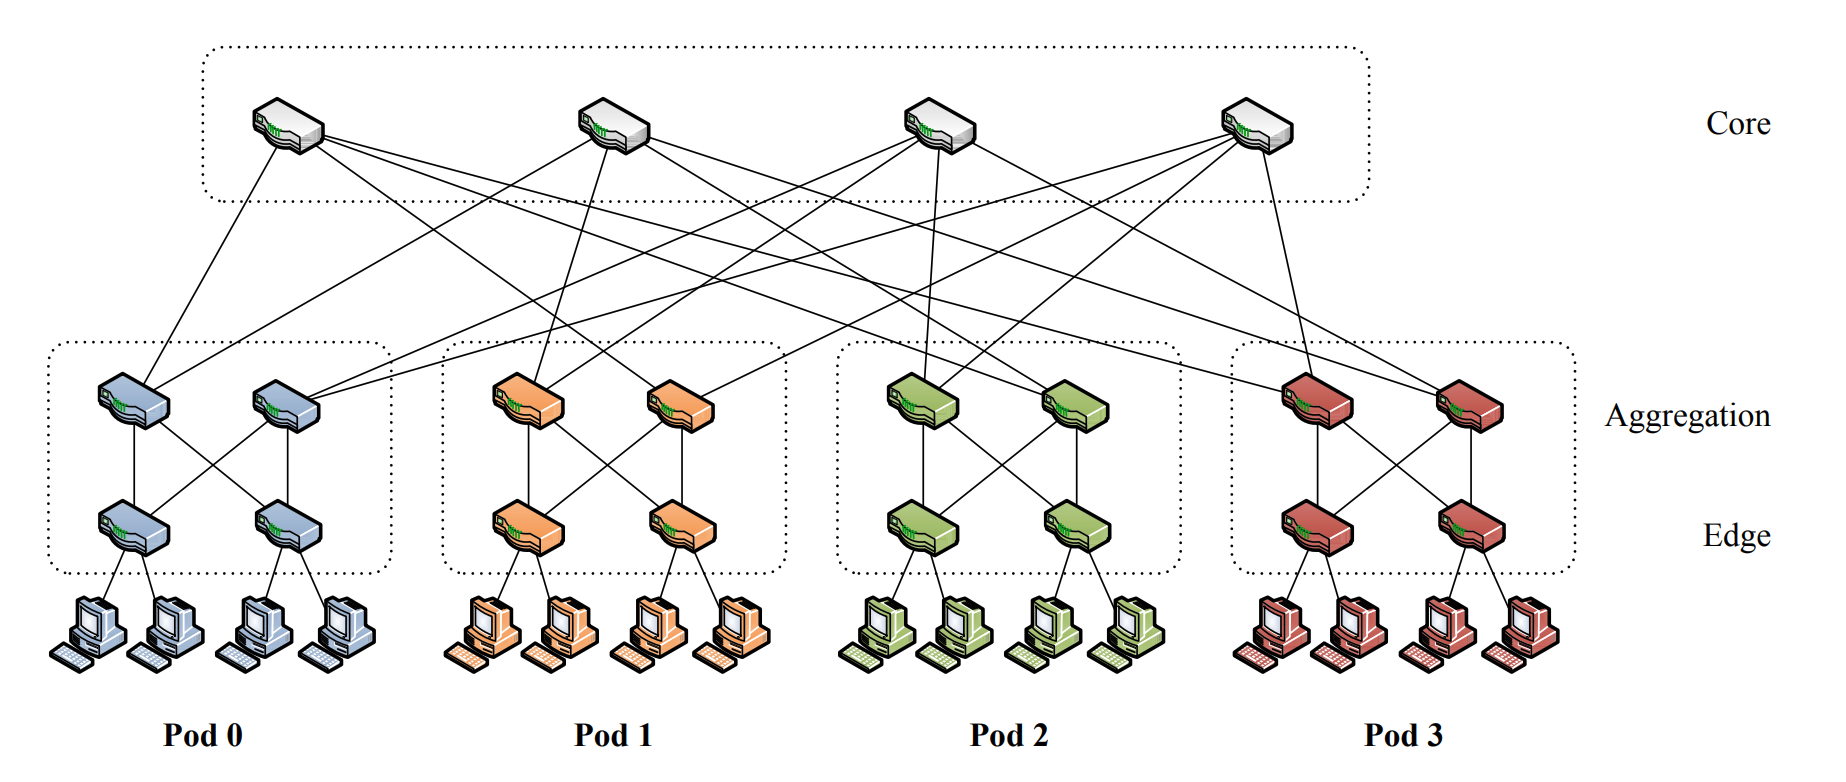
\includegraphics[width=0.75\textwidth]{figs/niranjan2009portland-1.png}

    \begin{itemize}
        \item How should flows be routed from nodes $i$ to $j$...

              \begin{itemize}
                  \item to minimize latency
                  \item to maximize bandwidth
                  \item to be maximally robust to failures
              \end{itemize}

    \end{itemize}

    \blfootcite{niranjan2009portland}
\end{frame}

\begin{frame}{Jupiter traffic engineering}
    \begin{itemize}
        \item input: $\approx 10$ aggregation blocks
        \item input: a bundle of parallel links between blocks
        \item input: predicted traffic matrix between blocks
        \item constraint: flows must reach destination within $2$ hops (latency)
        \item output: ???
    \end{itemize}

    \blfootcite{poutievski2022jupiter}
\end{frame}

\animation[poutievski2022jupiter]{Ex: Jupiter traffic engineering}
{figs/poutievski2022jupiter-3.pdf}
{
    figs/poutievski2022jupiter-1.pdf,
    figs/poutievski2022jupiter-2.pdf,
    figs/poutievski2022jupiter-3.pdf,
}

\begin{frame}{Jupiter traffic engineering (cont.)}
    \begin{itemize}
        \item def: a commodity $(s, t, d)$ is a demand $d$ between blocks $s$ and $t$
        \item input: a network $G = (V, E)$, capacities $c_e$, commodities $(s_k, t_k, d_k)$
        \item decision variables: for every $p: s_k \rightsquigarrow t_k$
              \begin{itemize}
                  \item $x^k_p$ the load commodity $k$ should put on on path $p$
              \end{itemize}
        \item objective: minimize max-utilization $U$ on any arc
    \end{itemize}

    \blfootcite{poutievski2022jupiter}
\end{frame}

\begin{frame}{Jupiter traffic engineering (cont.)}
    \begin{align*}
        \min_{x, U} \qquad & U                                                                  \\
        \text{s.t.} \qquad & \sum_{p \in P_k} x^k_p = d_k   \qquad \forall k                    \\
                           & \sum_k \sum_{p \in P_k : e \in p} x^k_p \le U c_e \qquad \forall e \\
                           & x^k_p \ge 0                    \qquad \forall p \in P_k
    \end{align*}

    \blfootcite{poutievski2022jupiter}
\end{frame}

\begin{frame}{Jupiter traffic engineering (cont.)}
    \centering
    \includegraphics[width=0.5\textwidth]{figs/poutievski2022jupiter-4.pdf}

    \begin{itemize}
        \item Robustness to inaccurate predictions
        \item Maximum-utilization for (a) is 1
        \item Maximum-utilization for (b) is 0.75
    \end{itemize}

    \blfootcite{poutievski2022jupiter}
\end{frame}

\begin{frame}{Jupiter traffic engineering (cont.)}
    \begin{itemize}
        \item Hyper-parameter $S \in (0, 1]$
    \end{itemize}

    \vspace{-\baselineskip}

    \begin{align*}
        \min_{x, U} \qquad & U                                                                                                                                                   \\
        \text{s.t.} \qquad & \sum_{p \in P_k} x^k_p = d_k   \qquad \forall k                                                                                                     \\
                           & \sum_k \sum_{p \in P_k : e \in p} x^k_p \le U c_e \qquad \forall e                                                                                  \\
                           & \textcolor{orange}{x^k_p \le d_k \frac{ \min_{e \in p} c_e }{ \sum_{q \in P_k} \min_{e \in q} c_e } \ab( \frac{1}{S} ) \qquad \forall k, p \in P_k} \\
                           & x^k_p \ge 0                    \qquad \forall k, p \in P_k
    \end{align*}

    \blfootcite{poutievski2022jupiter}
\end{frame}

\begin{frame}{Your turn!}
    \centering
    
\includegraphics[width=0.5\textwidth]{figs/colab_qrcode.jpeg}
    \url{https://colab.research.google.com/github/SIGma-UIUC/meetings/blob/main/FA26/Gurobi/notebook.ipynb}
\end{frame}

\section{Integer linear programs}
\frame{\tableofcontents[currentsection]}

\begin{frame}{bipartite matching}
    \begin{itemize}
        \item Given a bipartite graph $G = (L \cup R, E)$, find a maximum \emph{matching}.
    \end{itemize}

    \begin{align*}
        \max_{x} \qquad    & \sum_{e \in E} x_e                                           \\
        \text{s.t.} \qquad & \sum_{u \in N(v)} x_{uv} \le 1 \qquad \forall v \in L \cup R \\
                           & x_{uv} \in \set{0, 1}
    \end{align*}
\end{frame}

\begin{frame}{bipartite matching (cont.)}
    \begin{itemize}
        \item Given a bipartite graph $G = (L \cup R, E)$, find a maximum \emph{matching}.
    \end{itemize}

    \begin{align*}
        \max_{x} \qquad    & \sum_{e \in E} x_e                                           \\
        \text{s.t.} \qquad & \sum_{u \in N(v)} x_{uv} \le 1 \qquad \forall v \in L \cup R \\
                           & \textcolor{orange}{0 \le x_{uv} \le 1}
    \end{align*}

    \begin{itemize}
        \item Theorem: best fractional LP solution equals the best integer optimum
    \end{itemize}
\end{frame}

\begin{frame}{vertex cover}
    \begin{itemize}
        \item Given a graph $G = (V, E)$, find the smallest \emph{vertex cover}
    \end{itemize}

    \begin{align*}
        \min_{x} \qquad    & \sum_{v \in V} x_v                      \\
        \text{s.t.} \qquad & x_u + x_v \ge 1 \qquad \forall uv \in E \\
                           & x_v \in \set{0, 1}
    \end{align*}
\end{frame}

\begin{frame}{vertex cover (cont.)}
    \begin{itemize}
        \item Solving the LP relaxation:
    \end{itemize}

    \begin{align*}
        \min_{x} \qquad    & \sum_{v \in V} x_v                      \\
        \text{s.t.} \qquad & x_u + x_v \ge 1 \qquad \forall uv \in E \\
                           & \textcolor{orange}{0 \le x_v \le 1}
    \end{align*}

    \begin{itemize}
        \item So... how does this help us?
    \end{itemize}
\end{frame}

\begin{frame}{vertex cover (cont.)}
    \begin{itemize}
        \item Rounding a solution $x^*$ to the LP
        \item Let $\bar{x}_v = I(x^*_v \ge 1/2) \in \set{0, 1}$
        \item Satisfies $\bar{x}_v + \bar{x}_u \ge 1$ for each $uv \in E$
        \item 2-approximation: $\sum_{v \in V} \bar{x}_v \le 2 \sum_{v \in V} x^*_v \le 2 \text{OPT}$
    \end{itemize}
\end{frame}

\begin{frame}{independent set}
    \begin{itemize}
        \item Given a graph $G = (V, E)$, find the largest \emph{independent set}
    \end{itemize}

    \begin{align*}
        \max_{x} \qquad    & \sum_{v \in V} x_v                      \\
        \text{s.t.} \qquad & x_u + x_v \le 1 \qquad \forall uv \in E \\
                           & x_v \in \set{0, 1}
    \end{align*}
\end{frame}

\begin{frame}{independent set (cont.)}
    \begin{itemize}
        \item Solving the LP relaxation:
    \end{itemize}

    \begin{align*}
        \max_{x} \qquad    & \sum_{v \in V} x_v                      \\
        \text{s.t.} \qquad & x_u + x_v \le 1 \qquad \forall uv \in E \\
                           & \textcolor{orange}{0 \le x_v \le 1}
    \end{align*}
\end{frame}

\begin{frame}{independent set (cont.)}
    \begin{itemize}
        \item Suppose $G = K_n$, then maximum independent set has $1$ vertex
        \item obs: LP solution is at least $n/2$
        \item proof: let $x_v = 1/2$ for all vertices
        \item no (easy) way to \emph{round} the LP to be integral
    \end{itemize}
\end{frame}

\section{Branch and Bound}
\frame{\tableofcontents[currentsection]}

\begin{frame}{General form of integer linear program}
    \begin{align*}
        \min \qquad        & \vb{c}^T \vb{x}     \\
        \text{s.t.} \qquad & A \vb{x} \le \vb{b} \\
                           & x_i \in \Z
    \end{align*}

    \vspace{-\baselineskip}
    $$
        \Downarrow
    $$
    \vspace{-\baselineskip}

    \begin{align*}
        \min \qquad        & \vb{c}^T \vb{x}                       \\
        \text{s.t.} \qquad & A \vb{x} \le \vb{b}                   \\
                           & \textcolor{orange}{x_i \in \set{0,1}}
    \end{align*}
\end{frame}

\begin{frame}{Na\"ivety}
    \begin{columns}
        \begin{column}{0.5\textwidth}
            \begin{itemize}
                \item Enumerate all $2^n$ possible assignments
                \item Find the best out of all feasible solutions
            \end{itemize}

            \begin{align*}
                \min \qquad        & {-6x_1} - 2x_2 - 5x_3 - 2x_4   \\
                \text{s.t.} \qquad & 3x_1 + 2x_2 + 2x_3 + x_4 \le 4 \\
                                   & x_i \in \set{0, 1}
            \end{align*}
        \end{column}
        \begin{column}{0.5\textwidth}
            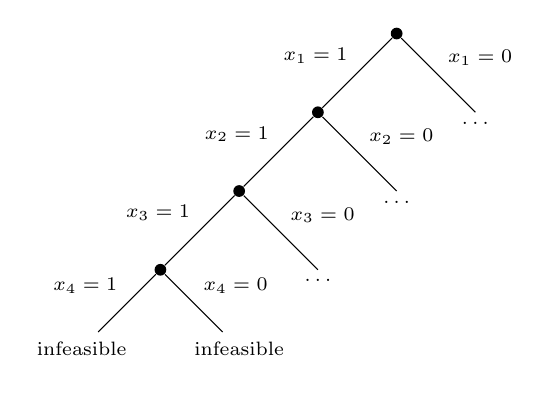
\begin{tikzpicture}[
                    every node/.style={font=\scriptsize},
                    dot/.style={circle, fill, inner sep=1.5pt},
                ]
                \node[dot] (r) at (0, 0) {};
                \node[dot] (a) at (-1, -1) {};
                \node[dot] (b) at (-2, -2) {};
                \node[dot] (c) at (-3, -3) {};
                \node (d) at (-4, -4) {infeasible};
                \node (e) at (-2, -4) {infeasible};

                \draw (r) -- node[above left] {$x_1 = 1$} (a);
                \draw (a) -- node[above left] {$x_2 = 1$} (b);
                \draw (b) -- node[above left] {$x_3 = 1$} (c);
                \draw (c) -- node[above left] {$x_4 = 1$} (d);
                \draw (c) -- node[above right] {$x_4 = 0$} (e);

                \draw (r) -- node[above right] {$x_1 = 0$} (1, -1) node[below] {$\dots$};
                \draw (a) -- node[above right] {$x_2 = 0$} (0, -2) node[below] {$\dots$};
                \draw (b) -- node[above right] {$x_3 = 0$} (-1, -3) node[below] {$\dots$};
            \end{tikzpicture}
        \end{column}
    \end{columns}
\end{frame}

\begin{frame}{Lower bounding and upper bounding solutions (min. problem)}
    \begin{itemize}
        \item LP relaxations lower bounds the true opt.
        \item Any found integral solution upper bounds the true solution
        \item Prune if a branch cannot beat the current best upper.
    \end{itemize}
\end{frame}

\begin{frame}{Branch-and-bound: pruning paths (example)}
    \begin{columns}
        \begin{column}{0.55\textwidth}
            \hspace*{-1cm}
            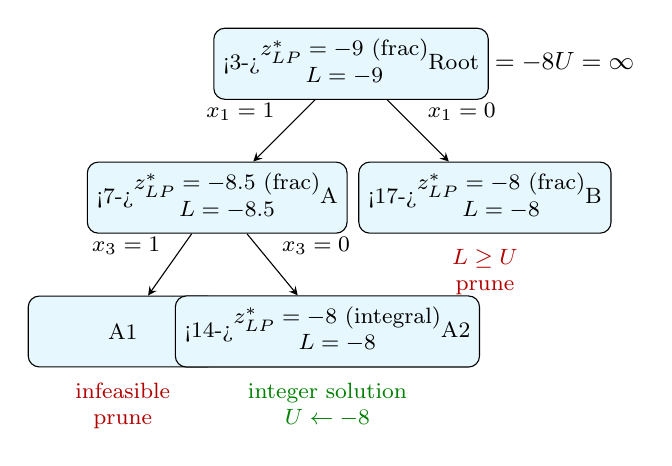
\begin{tikzpicture}[>=stealth, every node/.style={font=\footnotesize, align=center},
                    box/.style={draw, rounded corners, fill=cyan!10, minimum width=2.4cm, minimum height=0.9cm},
                    current/.style={draw=orange, very thick},
                    prune/.style={fill=gray!20}]
                \node[font=\small] at (2.2, 0) {\alt<14->{$U = -8$}{$U = \infty$}};

                \node[box, alt=<1-4>{current}{}] (r) at (0, 0)
                {\alt<3->{\begin{tabular}{@{}c@{}} $z^*_{LP} = -9$ (frac) \\ $L = -9$ \end{tabular}}{Root}};
                \node[box, visible on=<4->, alt=<5-8>{current}{}] (A) at (-1.7, -1.7)
                {\alt<7->{\begin{tabular}{@{}c@{}} $z^*_{LP} = -8.5$ (frac) \\ $L = -8.5$ \end{tabular}}{A}};
                \node[box, visible on=<4->, alt=<15-17>{current}{}, alt=<17->{prune}{}] (B) at (1.7, -1.7)
                {\alt<17->{\begin{tabular}{@{}c@{}} $z^*_{LP} = -8$ (frac) \\ $L = -8$ \end{tabular}}{B}};
                \node[box, visible on=<8->, alt=<9-11>{current}{}, alt=<11->{prune}{}] (A1) at (-2.9, -3.4) {A1};
                \node[box, visible on=<8->, alt=<12-14>{current}{}] (A2) at (-0.3, -3.4)
                {\alt<14->{\begin{tabular}{@{}c@{}} $z^*_{LP} = -8$ (integral) \\ $L = -8$ \end{tabular}}{A2}};

                \draw[->, visible on=<4->] (r) -- node[above left] {$x_1 = 1$} (A);
                \draw[->, visible on=<4->] (r) -- node[above right] {$x_1 = 0$} (B);
                \draw[->, visible on=<8->] (A) -- node[above left] {$x_3 = 1$} (A1);
                \draw[->, visible on=<8->] (A) -- node[above right] {$x_3 = 0$} (A2);

                \node[visible on=<11->, anchor=north, yshift=-2pt, text=red!70!black] at (A1.south)
                {infeasible \\ prune};
                \node[visible on=<14->, anchor=north, yshift=-2pt, text=green!50!black] at (A2.south)
                {integer solution \\ $U \gets -8$};
                \node[visible on=<17->, anchor=north, yshift=-2pt, text=red!70!black] at (B.south)
                {$L \ge U$ \\ prune};
            \end{tikzpicture}
        \end{column}
        \begin{column}{0.45\textwidth}
            \begin{overprint}
                \onslide<1-4>
                $L = -\infty < U = \infty$
                \visible<2->{
                    \knapsacklp{{-6x_1} - 2x_2 - 5x_3 - 2x_4}{3x_1 + 2x_2 + 2x_3 + x_4 \le 4}
                    $x^* = (\frac{1}{3}, 0, 1, 1)$, $z^*_{LP} = -9$
                }

                \visible<4->{Branch on $x_1$}

                \onslide<5-8>
                $L = -9 < U = \infty$
                \visible<6->{
                    \knapsacklp{{-6} - 2x_2 - 5x_3 - 2x_4}{2x_2 + 2x_3 + x_4 \le 1}
                    $x^* = (1, 0, \frac{1}{2}, 0)$, $z^*_{LP} = -8.5$
                }

                \visible<8->{Branch on $x_3$}

                \onslide<9-11>
                $L = -8.5 < U = \infty$
                \visible<10->{
                    \knapsacklp{{-11} - 2x_2 - 2x_4}{2x_2 + x_4 \le -1}
                    infeasible
                }

                \onslide<12-14>
                $L = -8.5 < U = \infty$
                \visible<13->{
                    \knapsacklp{{-6} - 2x_2 - 2x_4}{2x_2 + x_4 \le 1}
                    $x^* = (1, 0, 0, 1)$, $z^*_{LP} = -8$
                }

                \onslide<15-17>
                $L = -9 < U = -8$
                \visible<16->{
                    \knapsacklp{{-2x_2} - 5x_3 - 2x_4}{2x_2 + 2x_3 + x_4 \le 4}
                    $x^* = (0, \frac{1}{2}, 1, 1)$, $z^*_{LP} = -8$
                }

                \onslide<18>
                Optimal solution
                $$
                    x^* = (1, 0, 0, 1),
                    \qquad
                    U = -8
                $$
            \end{overprint}
        \end{column}
    \end{columns}
\end{frame}

\begin{frame}{Algorithmic loop}
    Branch-and-bound (minimization) problem for node $A$, given lower bound $L$ and best value $U$ thus far:

    \begin{itemize}
        \item If $L \ge U$, then quit (prune the branch).
        \item Find $(z^*_{LP}, x^*)$, update $L \gets \max(L, z^*_{LP})$.
        \item If $L \ge U$, then quit (prune the branch).
        \item If $x^*$ integral, update upper bound $U \gets z^*_{LP}$ and return $x^*$.
        \item Else branch on some fractional $x_j$, searching
              $$
                  x_j = 0,
                  \qquad
                  x_j = 1
              $$
              with local $L$ and the globally latest $U$.
    \end{itemize}
\end{frame}

\section{Traveling salesman}
\frame{\tableofcontents[currentsection]}

\begin{frame}{modeling}
    \begin{itemize}
        \item given a weighted digraph $G = (V, E, w)$, find the shortest tour visiting all nodes exactly once
        \item decision variables: $x_e \in \set{0, 1}$
        \item constraints: degree
              $$
                  \sum_{u \in N^-(v)} x_{u \to v} = 1
                  \qquad
                  \sum_{u \in N^+(v)} x_{v \to u} = 1
              $$
        \item constraints: connected
              \begin{itemize}
                  \item order vertices in increasing, according to the edges (excluding vertex 1)
                  \item decision variables $y_v$ for each $v$
                        $$
                            x_{u \to v} = 1 \implies y_v \ge y_u + 1
                        $$
                  \item representing as a linear constraint \footnotemark
                        \footnotetext{Gurobi has special ordered sets for this pattern; here we do it by hand}
                        $$
                            y_v - y_u - 1 \ge - n (1 - x_{uv})
                        $$
              \end{itemize}
    \end{itemize}
\end{frame}

\begin{frame}{formulation strength}
    \begin{itemize}
        \item large integrality gap: very small relaxed solutions means weak bounds
        \item enforce stronger topological constraints on the tour:
              \begin{itemize}
                  \item For each $ \emptyset \subsetneq S \subsetneq V$, then at least one edge entering/leaving $S$
              \end{itemize}
        \item much stronger constraints (smaller integrality gap)\footnotemark, but now we have exponentially many constraints to check
              \footnotetext{in fact, if TSP weights are a metric, then LP is provable $3/2$-approximation}
    \end{itemize}
\end{frame}

\begin{frame}{lazy constraints}
    \centering
    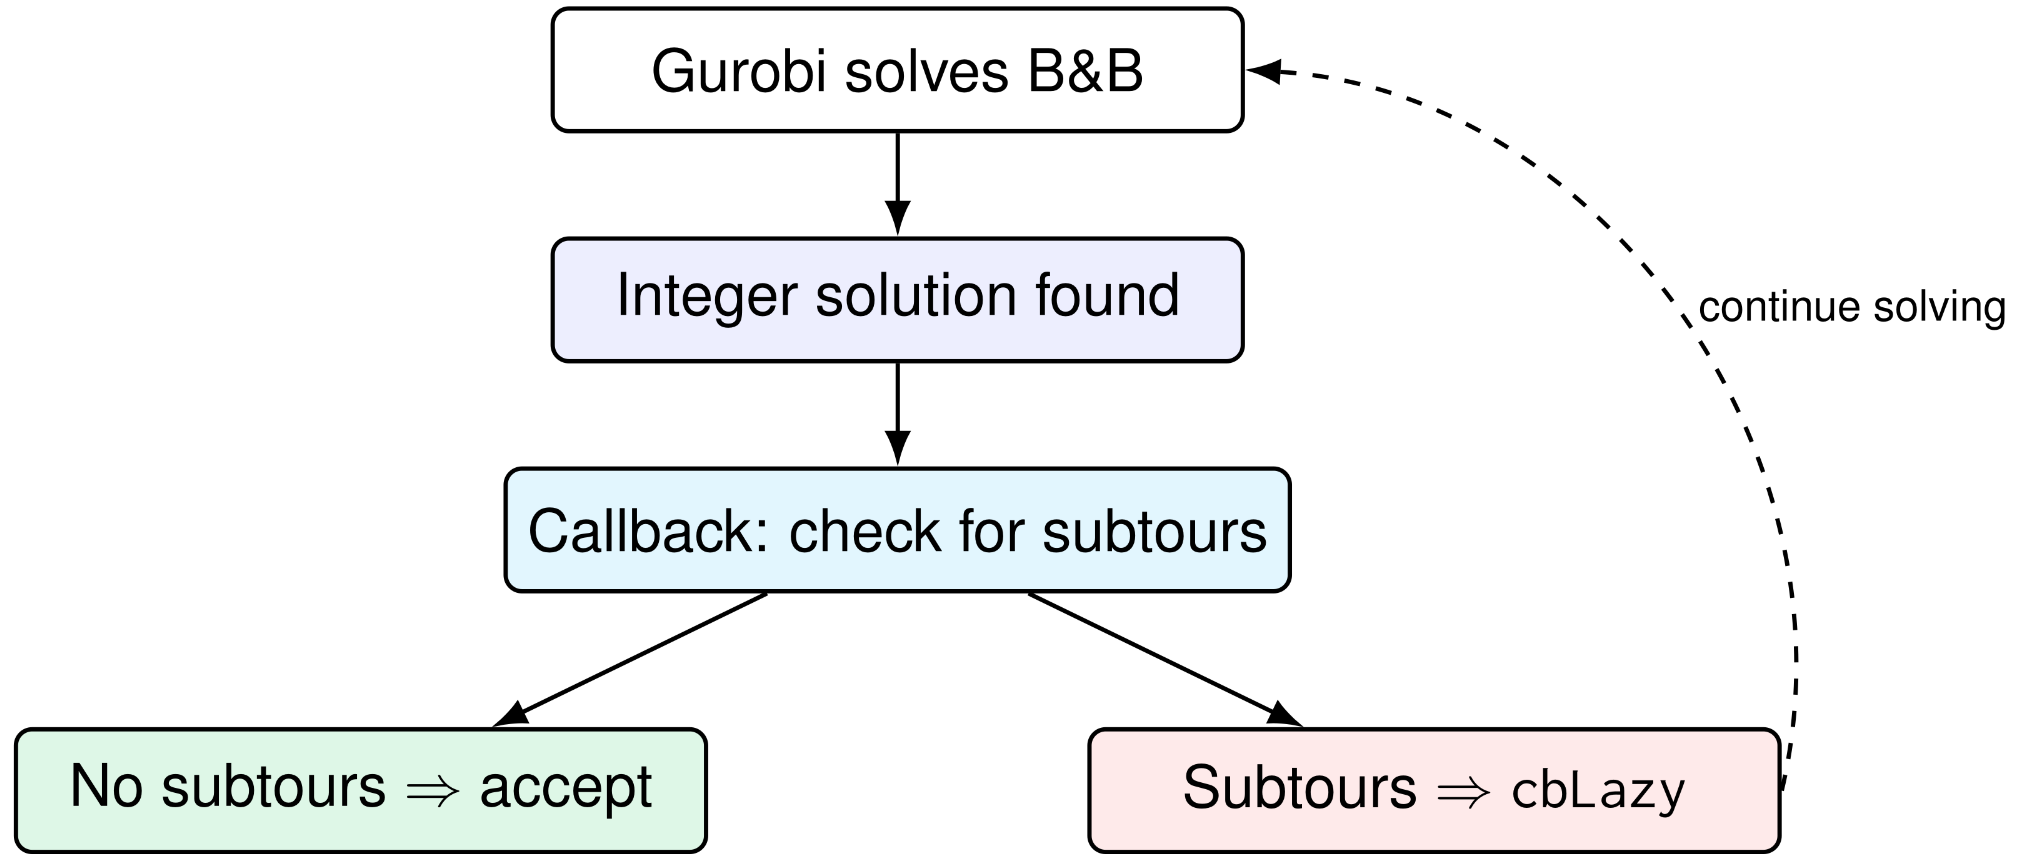
\includegraphics[width=\textwidth]{figs/farouk2026algorithmic-1.png}

    \blfootnote{From Spring 2026 CS498 AE}
\end{frame}

\begin{frame}{branch-and-cut}
    \centering
    \definecolor{bcfound}{HTML}{EDEEFE}
    \definecolor{bccallback}{HTML}{E2F6FE}
    \definecolor{bcbranch}{HTML}{DEF7E7}
    \definecolor{bccut}{HTML}{FEEAEA}
    \begin{tikzpicture}[>=stealth, font=\sffamily\small,
            box/.style={draw, thick, rounded corners, minimum width=4.2cm, minimum height=0.65cm},
            back/.style={->, thick, dashed}]
        \node[box, fill=white] (solve) at (0, 0) {Gurobi solves B\&B};
        \node[box, fill=bcfound] (found) at (0, -1.4) {Fractional solution found};
        \node[box, fill=bccallback] (callback) at (0, -2.8) {Callback: check for subtours};
        \node[box, fill=bcbranch] (branch) at (-3.2, -4.2) {No subtours $\Rightarrow$ branch};
        \node[box, fill=bccut] (cut) at (3.2, -4.2) {Subtours $\Rightarrow$ \texttt{cbCut}};
        \draw[->, thick] (solve) -- (found);
        \draw[->, thick] (found) -- (callback);
        \draw[->, thick] (callback) -- (branch);
        \draw[->, thick] (callback) -- (cut);
        \draw[back] (branch.west) to[out=90, in=180] node[pos=0.35, left] {\scriptsize branch} (solve.west);
        \draw[back] (cut.east) to[out=90, in=0] node[pos=0.35, right] {\scriptsize re-solve LP} (solve.east);
    \end{tikzpicture}

    \blfootnote{Modified from Spring 2026 CS498 AE}
\end{frame}

\section{Conclusion}

\begin{frame}{Credits and further reading}
    \begin{itemize}
        \item Slides closely based on material from Farouk's CS 498 AE
        \item Gurobi reference manual: {\small \url{docs.gurobi.com/projects/optimizer/en/13.0/index.html}}
        \item TSP developments: {\small \emph{Cook, William J. In pursuit of the traveling salesman: mathematics at the limits of computation. Princeton university press, 2015.}}
        \item Google blog post on optimization: {\small \url{research.google/blog/google-research-2022-beyond-algorithmic-advances/}}
        \item Meta blog post on optimization: {\small \url{engineering.fb.com/2026/09/21/open-source/rebalancer-generic-high-performance-library-assignment-problems/}}
        \item LinkedIn blog post on optimization: {\small \url{www.linkedin.com/blog/engineering/scalability/dualip-solving-extreme-scale-linear-programs}}
    \end{itemize}
\end{frame}

% \appendix

% \section{Bonus: fast approximations to (metric) TSP}
% \frame{\tableofcontents[currentsection]}

% \begin{frame}{approx algos}
%     \begin{itemize}
%         \item MST 2-approx
%         \item Christofides 1.5-approx
%     \end{itemize}
% \end{frame}

% \begin{frame}{simulated annealing}
% \end{frame}

% \section{Bonus: how to do better on TSP}
% \frame{\tableofcontents[currentsection]}

% \begin{frame}{TSP Leaderboard}

% \end{frame}

% \begin{frame}{Hybrid approaches}
%     warm starting gurobi
% \end{frame}

% \begin{frame}{Local cuts}

% \end{frame}

% \begin{frame}{Combs and dominoes}

% \end{frame}

% \section{Bonus: how to solve an LP (and prove it!)}
% \frame{\tableofcontents[currentsection]}

% \begin{frame}{Polytopes}

% \end{frame}

% \begin{frame}{Simplex}

% \end{frame}

% \begin{frame}{Duality}

% \end{frame}

% \section{Bonus: incremental constraints for LPs}
% \frame{\tableofcontents[currentsection]}

% \begin{frame}{Path-formulation of $s$-$t$ cut}

% \end{frame}

\end{document}
